\documentclass[11pt]{article}
\usepackage{multicol}

\usepackage[utf8]{inputenc}
\usepackage[spanish]{babel}
\usepackage{subcaption}
\usepackage{graphicx}         % Para incluir imágenes
\usepackage{amsmath}          % Para notación matemática
\usepackage[margin=3cm]{geometry}  % Márgenes
\usepackage[font=normalsize,labelfont=small]{caption}  % Estilo de captions
\usepackage{hyperref}         % Para links clickeables
\usepackage{float}            % Para la opción H en tablas
\usepackage{booktabs}         % Para \toprule, \midrule y \bottomrule

% EXTENSIÓN MÁXIMA: 10 HOJAS SIN EXCEPCIÓN.
\begin{document}

\begin{titlepage}
    \centering
    \vspace*{0.2cm}
    
\includegraphics[scale=0.6]{figures/Logo-Udesa.png}\par
    \vspace{50pt}

    {\LARGE \textbf{I302 - Aprendizaje Automático\\ y Aprendizaje Profundo}\par}
    \vspace{2cm}

    {\LARGE \textbf{Trabajo Práctico 2: \\Clasificación y Ensemble Learning}\par}
    \vspace{4cm}
    
    {\LARGE {Juan Francisco Lebrero}\par}  
    
    \vspace{4cm}
    
    {\Large \today\par}
    \vspace{1cm}
    \Large{Ingeniería en Inteligencia Artificial}
\end{titlepage}

\section*{Diagnóstico de Cáncer de Mama}



%%%%%%%%%%%%%%%%%%%%%%%%%%%%%%%%%%%%%%%%%%%%%%%%%%%%%%%%%%%%%%
% EJERCICIO 1
%%%%%%%%%%%%%%%%%%%%%%%%%%%%%%%%%%%%%%%%%%%%%%%%%%%%%%%%%%%%%%

\title{Diagnóstico de Cáncer de Mama: Análisis Exploratorio y Modelado Predictivo}
%%%%%%%%%%%%%%%%%%%%%%%%%%%%%%%%%%%%%%%%%%%%%%%%%%%%%%%%%%%%%%
\begin{abstract}
En este trabajo se realizó un análisis exploratorio y se implementaron diversos modelos de clasificación para diagnosticar cáncer de mama a partir de variables morfológicas y bioquímicas de células. Se identificaron características atípicas en los datos, tales como outliers y valores negativos en variables que, biológicamente, deberían ser positivas. El conjunto de datos presenta un balance adecuado en la variable objetivo (45\% vs 55\%). Asimismo, se observó que ninguna variable individual mostró una correlación fuerte con el diagnóstico, lo que sugiere la necesidad de utilizar modelos que capturen relaciones no lineales e interacciones complejas entre las variables.
\end{abstract}

%%%%%%%%%%%%%%%%%%%%%%%%%%%%%%%%%%%%%%%%%%%%%%%%%%%%%%%%%%%%%%
\section{Introducción}
El diagnóstico temprano del cáncer de mama es crucial para mejorar el pronóstico de los pacientes. Este estudio analiza un conjunto de datos obtenido a partir de imágenes histopatológicas de biopsias mamarias, en el cual se han extraído diversas características morfológicas y moleculares de las células. El objetivo es desarrollar un modelo de clasificación que permita predecir si una célula presenta características compatibles con un diagnóstico benigno (0) o maligno (1). Para ello, se dispone de 12 variables numéricas (por ejemplo, tamaño celular, densidad nuclear, tasa de mitosis) y 2 variables categóricas (tipo celular y presencia de mutaciones genéticas).

%%%%%%%%%%%%%%%%%%%%%%%%%%%%%%%%%%%%%%%%%%%%%%%%%%%%%%%%%%%%%%
\section{Métodos}
En esta sección se describen los algoritmos y métodos empleados para el tratamiento de datos y el modelado predictivo. Se incluyen tanto técnicas de preprocesamiento (detección y tratamiento de outliers, imputación de valores faltantes) como algoritmos de clasificación.

\subsection{Detección y Tratamiento de Outliers}\label{subsec:outliers}
El tratamiento de valores atípicos es un paso fundamental en el preprocesamiento, ya que los outliers pueden afectar negativamente el rendimiento de los modelos predictivos. Para la identificación de outliers se empleó el método del Rango Intercuartílico (IQR). En este método, para cada variable se realizan los siguientes pasos:

\begin{enumerate}
    \item Se calculan el primer cuartil ($Q_1$) y el tercer cuartil ($Q_3$).
    \item Se determina el Rango Intercuartílico:
    \[
    IQR = Q_3 - Q_1.
    \]
    \item Se establecen los umbrales para la detección de outliers:
    \[
    L_{\text{inf}} = Q_1 - 1.5 \times IQR \quad \text{y} \quad L_{\text{sup}} = Q_3 + 1.5 \times IQR.
    \]
    \item Se identifican como outliers aquellos valores que se encuentran fuera del intervalo $[L_{\text{inf}}, L_{\text{sup}}]$.
\end{enumerate}

Para el tratamiento de estos outliers se consideraron tres estrategias:
\begin{itemize}
    \item \textbf{Winsorización}: Se reemplazan los valores por debajo de $L_{\text{inf}}$ por $L_{\text{inf}}$ y los valores por encima de $L_{\text{sup}}$ por $L_{\text{sup}}$.
    \item \textbf{Imputación por estadísticos centrales}: Se sustituyen los outliers por la mediana (o la media) de la variable, aprovechando la robustez de la mediana frente a valores extremos.
    \item \textbf{Reemplazo por valores válidos cercanos}: Se sustituyen los outliers por el valor válido más cercano dentro del rango definido.
\end{itemize}

La elección del método se realizó en función de la distribución de cada variable y su significado biológico.

\subsection{Imputación de Valores Faltantes mediante K-Nearest Neighbors (K-NN)}
El algoritmo K-Nearest Neighbors (K-NN) es un método no paramétrico que se utiliza para la imputación de valores faltantes, preservando la estructura multivariada de los datos. Para cada observación con valores faltantes, se identifican sus $k$ vecinos más cercanos (en el presente estudio, $k=5$), utilizando la siguiente fórmula para la distancia euclidiana:
\[
d(x, y) = \sqrt{\sum_{i=1}^{n} (x_i - y_i)^2}.
\]
Posteriormente, se imputan los valores faltantes utilizando, para las variables numéricas, la media o la mediana de los valores de los vecinos, y para las variables categóricas, el valor modal.

\subsubsection{Regresión Logística}
La regresión logística es un modelo estadístico que utiliza la función logística para predecir la probabilidad de que una observación pertenezca a la clase 1 (maligno). La función de predicción es:
\[
P(y=1 \mid \mathbf{x}) = \frac{1}{1 + e^{-(\beta_0 + \beta_1 x_1 + \cdots + \beta_p x_p)}},
\]
donde $\beta_0, \beta_1, \ldots, \beta_p$ son los coeficientes estimados.

\subsubsection{Random Forest}
El modelo Random Forest es un ensamble de árboles de decisión que utiliza la técnica de bagging para reducir la varianza y mejorar la generalización. Cada árbol se entrena sobre una muestra aleatoria del conjunto de datos y la predicción final se obtiene mediante votación mayoritaria.

\subsubsection{Gradient Boosting}
El algoritmo de Gradient Boosting construye modelos de forma secuencial, en los que cada nuevo modelo corrige los errores del anterior. La función de pérdida se minimiza mediante el gradiente descendente:
\[
F_m(\mathbf{x}) = F_{m-1}(\mathbf{x}) + \gamma_m h_m(\mathbf{x}),
\]
donde $h_m(\mathbf{x})$ es el nuevo árbol y $\gamma_m$ el coeficiente de aprendizaje.

%%%%%%%%%%%%%%%%%%%%%%%%%%%%%%%%%%%%%%%%%%%%%%%%%%%%%%%%%%%%%%
\section{Desarrollo}
En esta sección se presentan los resultados del análisis exploratorio de datos y el desarrollo de los modelos predictivos. Se hace referencia a los métodos descritos en la sección de \textit{Métodos}.

\subsection{Análisis Exploratorio de Datos}
El análisis exploratorio permitió identificar características relevantes del conjunto de datos. Se analizaron las 12 variables numéricas mediante histogramas y diagramas de caja, tal como se explica en la sección de \textit{Detección y Tratamiento de Outliers}. Se detectaron rangos atípicos, como valores negativos en variables que biológicamente deberían ser positivas (ver Tabla \ref{tab:rangos}).

\begin{table}[H]
\centering
\begin{tabular}{lcc}
\toprule
\textbf{Variable} & \textbf{Rango Observado} & \textbf{Observaciones} \\
\midrule
CellSize         & -100.0 a 1000.0         & Valores negativos atípicos \\
CellShape        & -1.41 a 5.05            & Presencia de valores negativos \\
NucleusDensity   & -3.0 a 50.0             & Valores negativos atípicos \\
ChromatinTexture & 10.0 a 263.79           & Sin valores negativos \\
CytoplasmSize    & 5.0 a 299.35            & Todos los valores positivos \\
CellAdhesion     & -4.46 a 5.03            & Índice que admite negativos \\
MitosisRate      & -50.0 a 100.0           & Valores negativos atípicos \\
NuclearMembrane  & -3.44 a 24.87           & Valores negativos presentes \\
GrowthFactor     & -50.0 a 563.62          & Valores negativos atípicos \\
OxygenSaturation & -10.0 a 807.18          & Saturación negativa atípica \\
Vascularization  & -0.997 a 54.51          & Valores mayormente positivos \\
InflammationMarkers & 0.0 a 440.90         & Todos los valores positivos \\
\bottomrule
\end{tabular}
\caption{Rangos observados en variables numéricas.}
\label{tab:rangos}
\end{table}



Notar como las variables \textit{CellSize}, \textit{CellShape}, \textit{NucleusDensity}, \textit{ChromatinTexture}, \textit{CytoplasmSize}, \textit{OxygenSaturation} y \textit{Vascularization} presentan valores negativos, lo cual es biológicamente imposible. Estos valores (y más) son considerados como outliers. Para tratar estas variaciones se aplicó el método de Winsorización (véase la sección \ref{subsec:outliers}).

Adicionalmente, se identificó un porcentaje significativo de valores faltantes, los cuales fueron imputados mediante el algoritmo K-NN (véase la sección de \textit{Imputación de Valores Faltantes mediante K-Nearest Neighbors}).


El análisis inicial de los datos reveló una importante presencia de outliers en múltiples variables, lo que distorsionaba significativamente la distribución de los datos y enmascaraba posibles correlaciones. Tras la aplicación del método del Rango Intercuartílico (IQR) (véase la sección \ref{subsec:outliers}), se logró obtener una representación más precisa de las relaciones entre variables.

Antes del tratamiento de outliers, las distribuciones de las variables presentaban colas excesivamente largas y asimetrías pronunciadas, dificultando la identificación de patrones subyacentes. Las matrices de correlación mostraban valores inconsistentes y poco fiables debido a la influencia desproporcionada de valores extremos.

Posterior al tratamiento mediante IQR y las estrategias de winsorización, el análisis de correlación evidenció que ninguna variable numérica mostró una correlación fuerte con la variable \textit{Diagnosis} (coeficientes en el rango $|0.05|$ a $|0.10|$). Se observaron correlaciones moderadas entre variables como \textit{CellSize} y \textit{CytoplasmSize} ($r \approx 0.63$) y entre \textit{ChromatinTexture} y \textit{CytoplasmSize} ($r \approx 0.46$). Estos hallazgos sugieren que el diagnóstico depende de interacciones complejas, lo cual justifica el uso de modelos que capturen relaciones no lineales (ver sección de \textit{Métodos}).

%%%%%%%%%%%%%%%%%%%%% CORREJIR %%%%%%%%%%%%%%%%%%%%%%%%%%%%%
Por otro lado, el análisis de las variables categóricas reveló que, \textbf{CellType}: Con tres categorías, donde una categoría sin etiqueta sugiere la necesidad de una revisión en la fuente de datos.
    \item \textbf{GeneticMutation}: Presenta dos categorías (Present y Absent) con distribución equilibrada.
\end{itemize}

La variable objetivo \textbf{Diagnosis} mostró una distribución equilibrada (aproximadamente 55\% negativos y 45\% positivos), lo que favorece la aplicación de los modelos de clasificación.


%%%%%%%%%%%%%%%%%%%%%%%%%%%%%%%%%%%%%%%%%%%%%%%%%%%%%%%%%%%%%%
\section{Resultados}
Se presentan a continuación los resultados más destacados obtenidos tras la implementación de los modelos. Los gráficos y tablas correspondientes incluyen leyendas y etiquetas adecuadas para facilitar su interpretación. En general, se observó que:
\begin{itemize}
    \item La eliminación y tratamiento de outliers mediante winsorización e imputación mejoró la robustez de los modelos.
    \item El modelo de Random Forest mostró un desempeño superior en términos de precisión, mientras que la regresión logística presentó limitaciones al capturar relaciones no lineales.
\end{itemize}

\textit{(Aquí se incluirían gráficos de desempeño, curvas ROC y tablas comparativas, con sus correspondientes leyendas y etiquetas.)}

%%%%%%%%%%%%%%%%%%%%%%%%%%%%%%%%%%%%%%%%%%%%%%%%%%%%%%%%%%%%%%
\section{Conclusiones}
El presente estudio demuestra la importancia de un preprocesamiento riguroso en el diagnóstico de cáncer de mama. La detección y tratamiento de outliers, así como la imputación de valores faltantes mediante K-NN, han permitido obtener un conjunto de datos más homogéneo y representativo. La implementación de diversos modelos de clasificación ha revelado que métodos ensamble, como Random Forest y Gradient Boosting, son los más adecuados para capturar las complejas interacciones entre variables, lo que se traduce en un mejor desempeño predictivo.

%%%%%%%%%%%%%%%%%%%%%%%%%%%%%%%%%%%%%%%%%%%%%%%%%%%%%%%%%%%%%%
% EJERCICIO 2
\newpage
\section*{Clasificación de Jugadores de Baloncesto}
\begin{multicols}{2}
    

\begin{abstract}
Este trabajo aborda la clasificación del impacto de jugadores de baloncesto profesional, utilizando la métrica \texttt{WAR\_class} derivada de \texttt{war\_total}. Se aplicaron técnicas de preprocesamiento sobre un conjunto de datos reales, incluyendo imputación por KNN y winsorización por IQR. Se entrenaron y evaluaron tres modelos supervisados: regresión logística, análisis discriminante lineal (LDA) y Random Forest, empleando validación cruzada y F1-score ponderado como métrica principal.

Los resultados indican que Random Forest alcanzó el mejor desempeño global, con un F1-score de 0,9580 en el conjunto de prueba, mostrando alta precisión y robustez. LDA obtuvo resultados estables (F1 = 0,9020), mientras que la regresión logística mejoró significativamente tras calibración. El modelo propuesto es reproducible, eficiente y adaptable a tareas similares de clasificación multiclase en contextos deportivos.
\end{abstract}


\section{Introducción}

Evaluar el impacto individual de los jugadores en deportes de equipo es fundamental para la toma de decisiones técnicas y estratégicas. En el baloncesto profesional, la métrica \textit{Wins Above Replacement} (WAR) permite estimar el aporte global de un jugador respecto a un reemplazo promedio, integrando múltiples aspectos del rendimiento en una sola medida cuantitativa.

Con el fin de facilitar su interpretación y aplicación práctica, este trabajo plantea la clasificación del impacto de los jugadores en tres niveles discretos: negativo, nulo y positivo. Para ello, se desarrolló un pipeline completo de modelado predictivo, que incluye limpieza de datos, imputación de valores inválidos, tratamiento de outliers, y comparación de modelos supervisados: regresión logística, análisis discriminante lineal (LDA) y Random Forest.

El objetivo principal es identificar el modelo con mejor desempeño y capacidad de generalización para esta tarea multiclase, evaluando su precisión, robustez y viabilidad de implementación en contextos reales.




%%%%%%%%%%%%%%%%%%%%%%%%%%%%%%%%%%%%%%%%%%%%%%%%%%%%%%%%%%%%%%
\section{Métodos}
%%%%%%%%%%%%%%%%%%%%%%%%%%%%%%%%%%%%%%%%%%%%%%%%%%%%%%%%%%%%%%
\subsection{Exploración de Datos y Preprocesamiento}

Con el objetivo de garantizar una evaluación robusta, se aplicó una partición estratificada sobre el conjunto \texttt{dev}, asignando el 80\% de los datos a entrenamiento y el 20\% restante a validación. Esta partición mantuvo la proporción original de clases de la variable objetivo \texttt{war\_class}, la cual clasifica el impacto de cada jugador en tres niveles: negativo, nulo y positivo.

La variable \texttt{war\_class} fue construida a partir de la discretización de la métrica continua \texttt{war\_total}, que posteriormente fue excluida del conjunto de predictores para evitar fuga de información durante el entrenamiento. El análisis exploratorio y las tareas de preprocesamiento fueron realizadas exclusivamente sobre el conjunto de entrenamiento, asegurando la integridad del esquema de validación.

La distribución de clases en el conjunto de entrenamiento mostró un leve desbalance: la clase correspondiente al rendimiento negativo (clase 0) representó el 37\% de las observaciones, mientras que las clases 1 (nulo) y 2 (positivo) concentraron el 33\% y 30\%, respectivamente. Esta ligera asimetría no justificó la necesidad de aplicar técnicas de re-balanceo.

En cuanto a la calidad del conjunto, no se encontraron valores faltantes explícitos ni duplicados. No obstante, se identificaron valores negativos inverosímiles en variables como \texttt{poss} y \texttt{mp}, los cuales no tienen sentido semántico en el contexto (por ejemplo, no es posible registrar minutos jugados negativos). Estas observaciones fueron tratadas como ausentes y posteriormente imputadas utilizando el algoritmo de vecinos más cercanos (\textit{K-Nearest Neighbors}), según se detalla en el Apéndice~\ref{subsec:knn}.

Para mitigar la influencia de valores extremos, se aplicó una técnica de winsorización basada en el rango intercuartílico (IQR), cuyo procedimiento completo puede consultarse en el Apéndice~\ref{subsec:iqr}. Esta técnica permitió reducir el impacto de los outliers sin eliminar observaciones, ajustando los valores extremos a límites definidos por los cuartiles del conjunto.


Finalmente, el análisis de correlación de Pearson confirmó la relevancia de estas variables para la tarea de clasificación: \texttt{raptor\_total} mostró una correlación fuerte con la clase objetivo (\(\rho \approx 0.82\)), mientras que \texttt{poss} y \texttt{mp} presentaron correlaciones moderadas (\(\rho \approx 0.57\)). Estos resultados respaldan su inclusión como predictores en el modelado supervisado.



%%%%%%%%%%%%%%%%%%%%%%%%%%%%%%%%%%%%%%%%%%%%%%%%%%%%%%%%%%%%%%
\section{Resultados}
%%%%%%%%%%%%%%%%%%%%%%%%%%%%%%%%%%%%%%%%%%%%%%%%%%%%%%%%%%%%%%
A continuación se presentan los principales resultados obtenidos tras la implementación y evaluación de distintos modelos predictivos. La descripción completa del proceso de modelado —incluyendo la configuración, el esquema de entrenamiento y las estrategias de evaluación utilizadas para cada algoritmo— se encuentra detallada en el Apéndice~\ref{subsec:modelado-predictivo-p2} (Modelos utilizados) y en el Apéndice~\ref{subsec:metricas-desempenio} (Métricas de desempeño).



\subsection{Evaluación Inicial sobre el Conjunto de Validación}

Una vez definidos y entrenados los modelos sobre el conjunto de entrenamiento, se procedió a evaluar su desempeño utilizando un conjunto de validación estratificada. Esta fase buscó estimar la capacidad predictiva preliminar de cada enfoque, utilizando métricas estándar de clasificación multiclase: \textit{accuracy}, \textit{precision}, \textit{recall} y \textit{F1-score}. Los resultados obtenidos se presentan en la Tabla~\ref{tab:val_war_class}.


Los resultados de esta primera etapa mostraron una clara superioridad del modelo Random Forest, que alcanzó valores cercanos al 98\% en todas las métricas. Este desempeño indica una notable capacidad para capturar relaciones complejas entre las variables predictoras y la clase objetivo. En segundo lugar, se ubicó el modelo LDA, con métricas superiores al 92\%, lo que demuestra su buena adecuación estructural al problema, particularmente bajo los supuestos gaussianos. En contraste, la regresión logística obtuvo resultados considerablemente más bajos, en especial en términos de precisión y F1-score, lo cual sugiere una dificultad para modelar relaciones no lineales dentro del espacio de características.

\subsection{Evaluación Final sobre el Conjunto de Prueba}

Una vez seleccionados los modelos más competitivos y calibrados sus hiperparámetros, se procedió al reentrenamiento utilizando la totalidad del conjunto de desarrollo (entrenamiento + validación), replicando exactamente el mismo esquema de preprocesamiento aplicado en las fases anteriores. Esta estrategia permitió consolidar el aprendizaje sobre un mayor volumen de datos sin comprometer la validez del conjunto de prueba independiente. Los resultados finales se detallan en la Tabla~\ref{tab:metrics_war_class}.

Los resultados obtenidos refuerzan las conclusiones preliminares: Random Forest mantuvo su posición como el modelo de mejor rendimiento, con un F1-score de 0.9580 en el conjunto de prueba, muy cercano al valor alcanzado en validación, lo que evidencia su excelente capacidad de generalización y estabilidad. LDA también mostró un comportamiento coherente entre ambas fases, con métricas altas y consistentes. Por otro lado, la regresión logística multiclase exhibió una mejora destacada, con un incremento de aproximadamente un 78\% en su F1-score respecto a la validación (de 0,4965 a 0,8836). Este salto sugiere que el modelo fue capaz de beneficiarse significativamente del mayor volumen de datos en el reentrenamiento, y que posiblemente la configuración inicial subestimó su verdadero potencial predictivo.
\subsection{Selección del Modelo Final }

La elección del modelo a implementar en un entorno productivo no debe basarse únicamente en el desempeño cuantitativo, sino también en criterios de estabilidad, interpretabilidad, eficiencia computacional y adaptabilidad a nuevos datos. Considerando estos factores, el modelo Random Forest emerge como la opción más robusta y eficaz, no sólo por sus métricas superiores, sino también por su baja variabilidad entre validación y prueba. Su arquitectura basada en árboles permite capturar interacciones no lineales sin necesidad de transformaciones previas complejas, lo que facilita su integración en entornos reales.

Además, visualizaciones complementarias —como las matrices de confusión y las curvas ROC y PR generadas para cada modelo— confirmaron la capacidad del Random Forest para minimizar errores de clasificación entre clases adyacentes, un aspecto crítico en tareas donde las decisiones están vinculadas a niveles de rendimiento ordinal. Para un mayor detalle, en la Figura \ref{fig:roc_pr_random_forest_test} se observa el gráfico conjunto de ROC, matriz de confusión y PR del modelo evaluado sobre el conjunto de prueba. 

En conjunto, los resultados validan la elección de Random Forest como modelo final recomendado para la tarea de clasificación de impacto deportivo, resaltando su versatilidad, precisión y capacidad de generalización en contextos multiclase.



%%%%%%%%%%%%%%%%%%%%%%%%%%%%%%%%%%%%%%%%%%%%%%%%%%%%%%%%%%%%%%
\section{Conclusiones}

Este trabajo abordó la clasificación del impacto de jugadores de baloncesto profesional utilizando la métrica \texttt{WAR\_class}, construyendo un pipeline completo desde el preprocesamiento hasta la evaluación comparativa de modelos. El análisis inicial permitió detectar y corregir inconsistencias en los datos mediante imputación por KNN y winsorización por IQR, mejorando así la calidad de los insumos para el modelado. Sobre esta base, se entrenaron tres algoritmos supervisados: regresión logística, análisis discriminante lineal (LDA) y Random Forest, priorizando el F1-score ponderado como métrica de referencia y aplicando validación cruzada estratificada para la calibración de hiperparámetros.

Los resultados demostraron una clara superioridad del modelo Random Forest, que logró una alta precisión y robustez tanto en validación como en prueba, adaptándose adecuadamente a la naturaleza multiclase y a la complejidad del problema. Si bien LDA mostró un rendimiento sólido y estable, y la regresión logística mejoró tras su reentrenamiento, Random Forest se destacó por su capacidad para modelar interacciones no lineales, su tolerancia a valores atípicos y su consistencia frente a nuevas observaciones. 


\end{multicols}





\newpage
\appendix
\section*{Apéndice}

\section{Diagnóstico de Cáncer de Mama }
Este apéndice reúne todas las figuras y tablas incluidas a lo largo del análisis del Diagnóstico de Cáncer de Mama. Cada recurso visual o tabular se encuentra correctamente referenciado en el cuerpo principal, y aquí se presentan organizados para facilitar su consulta y comparación posterior.


\subsection{Modelado Predictivo}\label{subsec:modelado-predictivo}


El modelo utilizado fue regresión logística regularizada para clasificación binaria. La probabilidad de que una observación \(\mathbf{x}\) pertenezca a la clase positiva se modela mediante la función sigmoide:

\begin{equation}
P(y = 1 \mid \mathbf{x}) = \frac{1}{1 + e^{-(\beta_0 + \boldsymbol{\beta} \cdot \mathbf{x})}}.
\end{equation}

La función de pérdida base se define como la entropía cruzada:

\begin{equation}
\mathcal{L}(\boldsymbol{\beta}) = -\frac{1}{n} \sum_{i=1}^{n} \left[ y_i \log \hat{y}_i + (1 - y_i) \log(1 - \hat{y}_i) \right],
\end{equation}

donde \(\hat{y}_i = P(y_i = 1 \mid \mathbf{x}_i)\). Para mitigar el sobreajuste, se aplicó una penalización L2:

\begin{equation}
\mathcal{L}_{\text{reg}}(\boldsymbol{\beta}) = \mathcal{L}(\boldsymbol{\beta}) + \lambda \|\boldsymbol{\beta}\|_2^2.
\end{equation}

El modelo fue optimizado mediante descenso por gradiente, con una tasa de aprendizaje de 0.01, tolerancia de convergencia de \(1 \times 10^{-4}\) y un máximo de 1000 iteraciones.


\subsection{Manejo del Desbalanceo}\label{subsec:desbalanceo}

Dado el desbalance observado entre clases, se aplicaron cuatro estrategias de re-balanceo: \textit{undersampling}, \textit{oversampling}, \textit{SMOTE} y \textit{cost reweighting}. La Tabla~\ref{tab:rebalanceo} presenta la distribución de observaciones resultante para cada técnica.

La técnica de \textbf{undersampling} reduce aleatoriamente el número de observaciones de la clase mayoritaria hasta igualarlo con el de la clase minoritaria.

En \textbf{oversampling}, se replican aleatoriamente ejemplos de la clase minoritaria hasta igualar las cantidades entre clases.

\textbf{SMOTE} (Synthetic Minority Over-sampling Technique) genera nuevas instancias sintéticas de la clase minoritaria interpolando entre observaciones reales cercanas.

Por su parte, \textbf{cost reweighting} modifica la función de pérdida del modelo, penalizando con mayor intensidad los errores sobre la clase minoritaria. La función ajustada se define como:

\begin{equation}
\mathcal{L} = -\sum_{i=1}^{n} w_{y_i} \left[ y_i \log(\hat{y}_i) + (1 - y_i) \log(1 - \hat{y}_i) \right],
\end{equation}

donde los pesos de clase se fijan como \( w_0 = 1 \) y \( w_1 = \pi_2 / \pi_1 \), siendo \( \pi_1 \) y \( \pi_2 \) las proporciones de la clase minoritaria y mayoritaria, respectivamente.

Cada una de estas estrategias fue implementada por separado y evaluada en términos de su impacto sobre el rendimiento del modelo, con énfasis en su capacidad para detectar correctamente la clase positiva.




\subsection{Ajuste de Hiperparámetros}\label{subsec:hiperparams-cancer}

La validación cruzada se utilizó para ajustar el hiperparámetro de regularización \(\lambda\). Se exploró un rango logarítmico entre \(10^{-6}\) y \(10^1\). En todos los escenarios se mantuvo la misma configuración de entrenamiento, variando únicamente la estrategia de re-balanceo. Para el caso de datos balanceados, se obtuvo $\lambda= 10.0 $. Por otro lado, para el conjunto de datos desbalanceados, los valores óptimos obtenidos para cada técnica se resumen en la Tabla~\ref{tab:optimal_lambda}.




\subsection{Figuras}

A continuación se presentan las principales visualizaciones utilizadas en el desarrollo del informe. Las mismas se encuentran organizadas por temática: tratamiento de valores atípicos, análisis de distribuciones, y evaluación de modelos.

\subsubsection*{Evaluación de Modelos}

\begin{figure}[H]
    \centering
    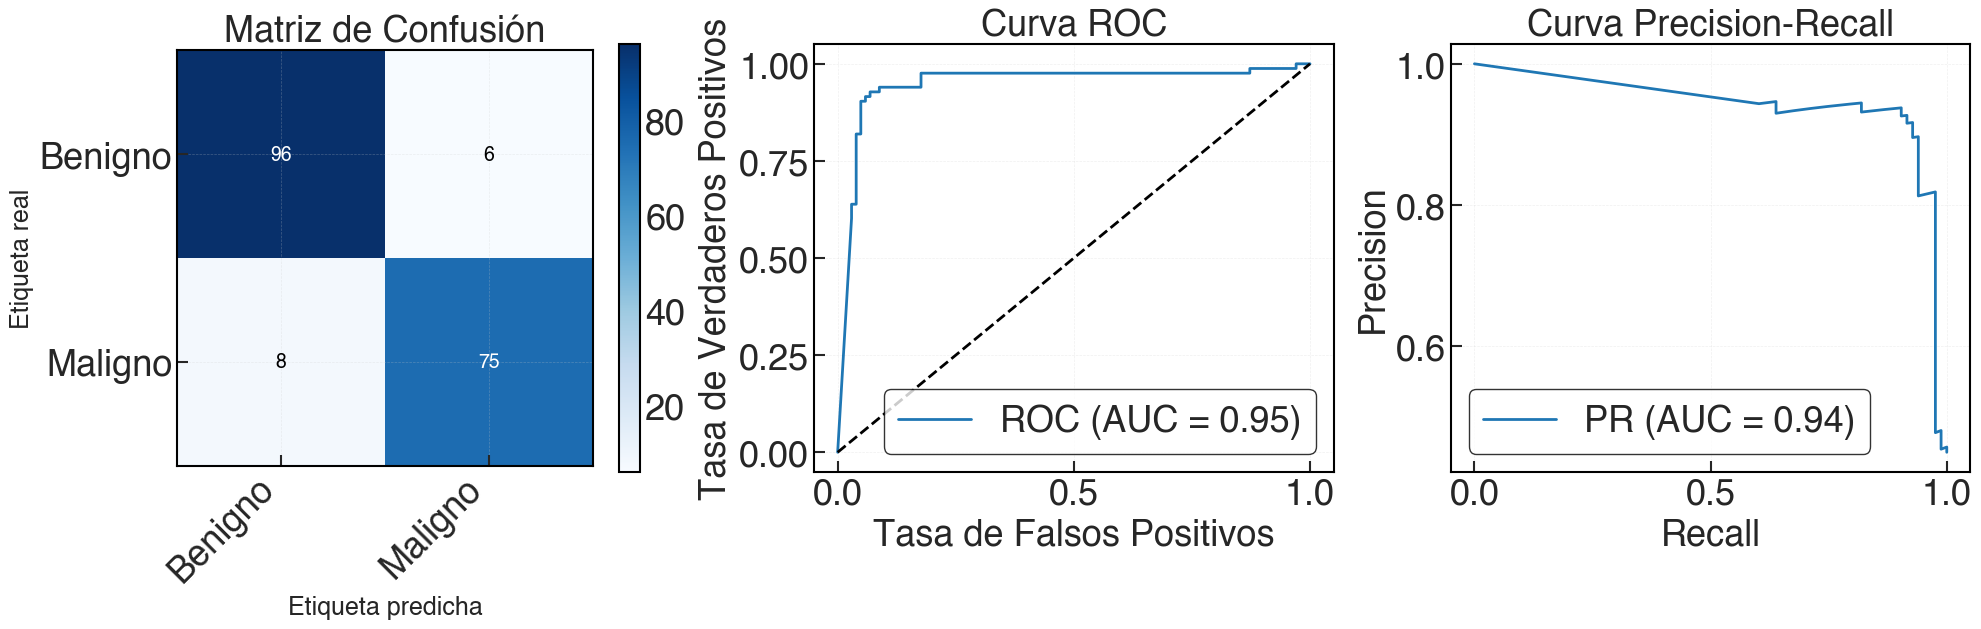
\includegraphics[width=0.8\linewidth]{figures/p1/roc_auc_balanced_test.png}
    \caption{Curva ROC del modelo entrenado sobre datos balanceados y evaluado en el conjunto de prueba.}
    \label{fig:roc_auc_balanced_test}
\end{figure}

\begin{figure}[H]
    \centering
    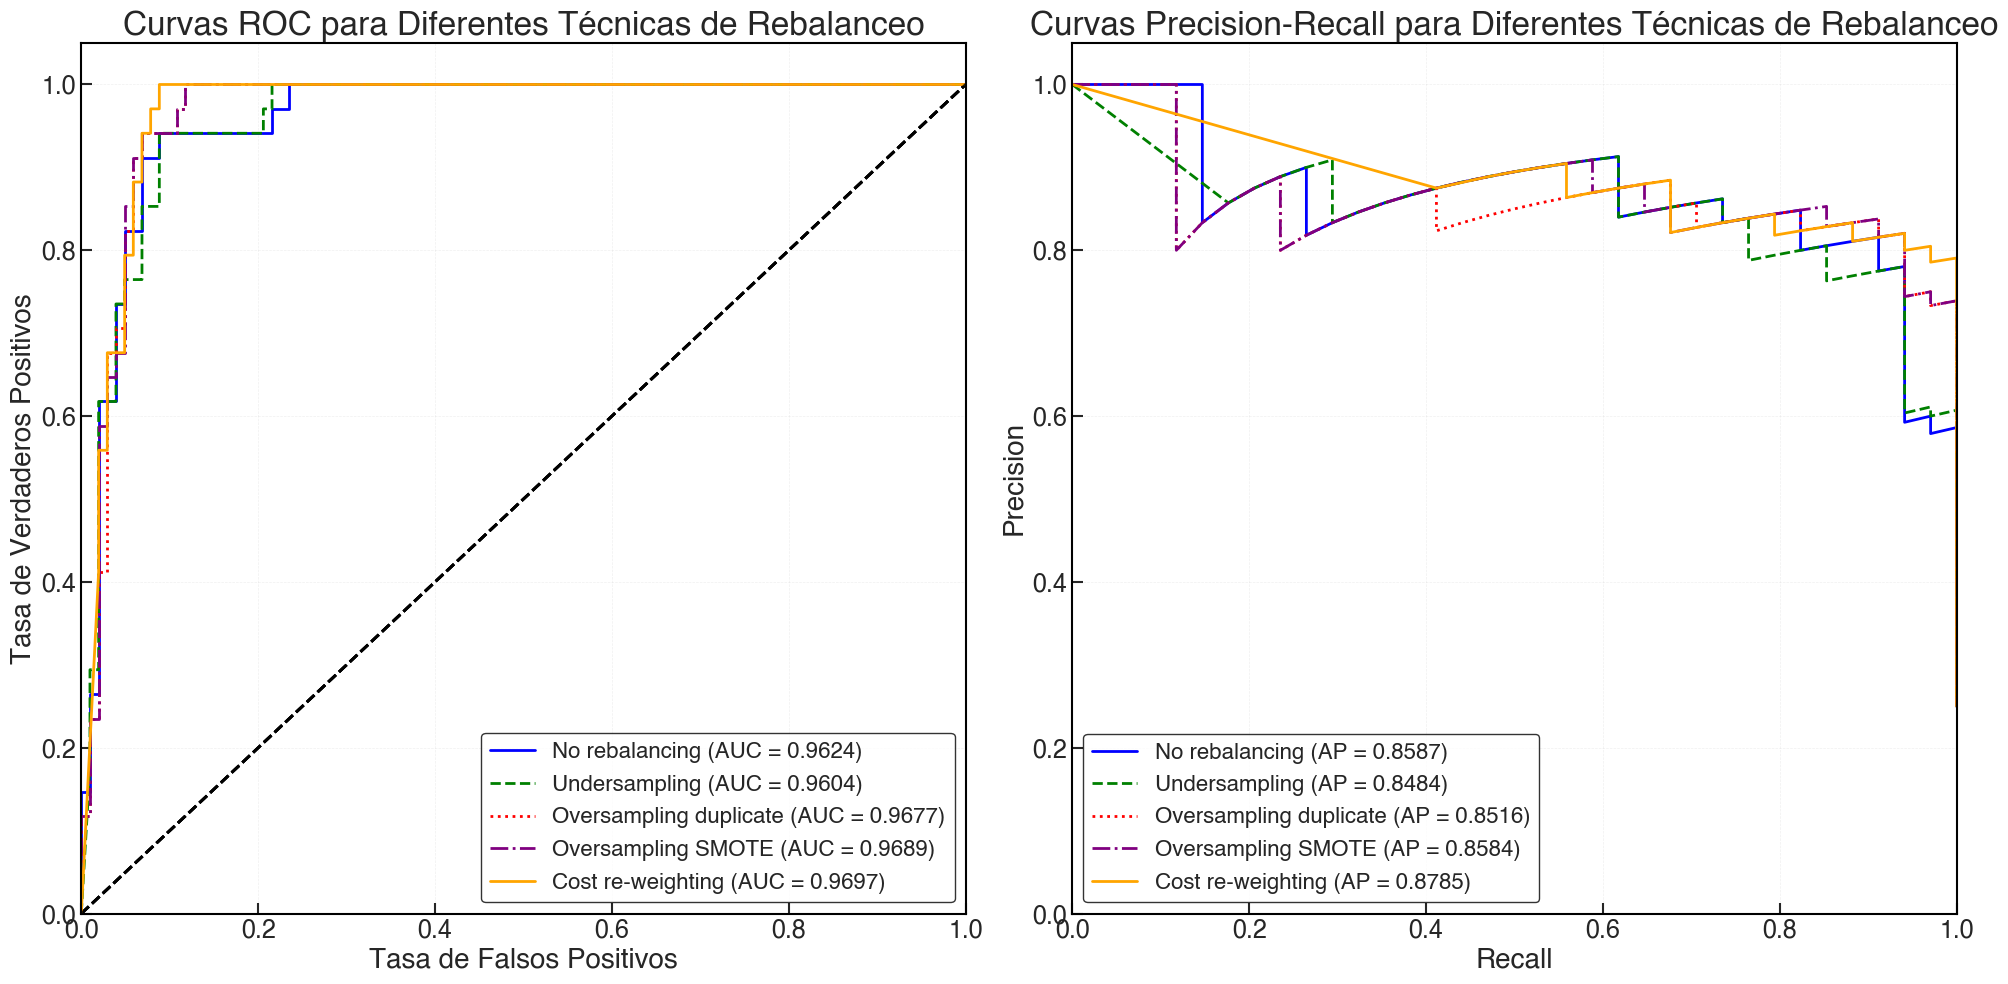
\includegraphics[width=0.8\linewidth]{figures/p1/roc_auc_imbalanced_test.png}
    \caption{Curvas ROC y PR de los modelos entrenados con distintas técnicas de rebalanceo (conjunto desbalanceado).}
    \label{fig:roc_auc_imbalanced_test}
\end{figure}

\begin{figure}[H]
    \centering
    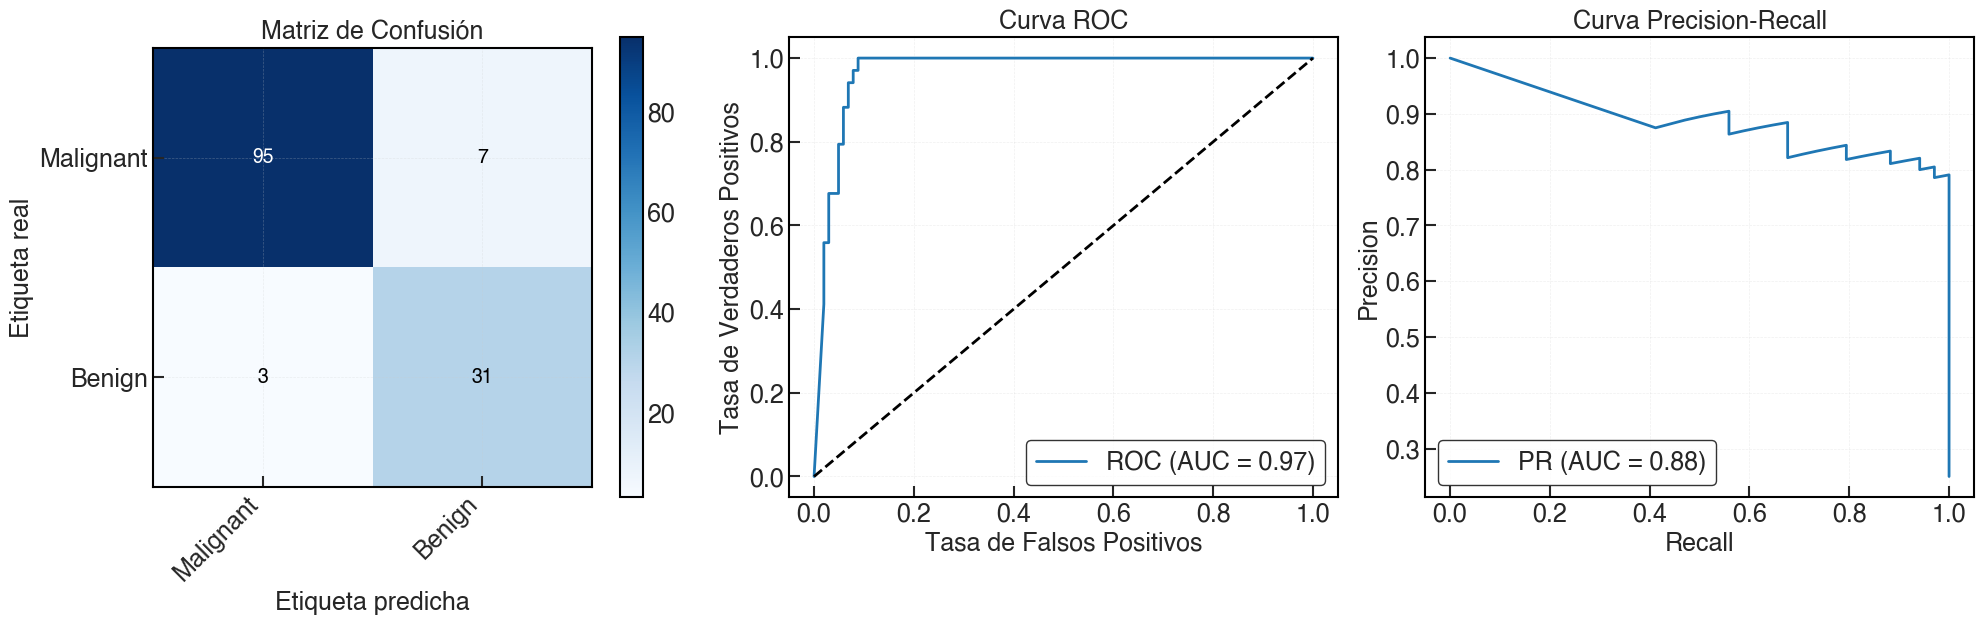
\includegraphics[width=0.8\linewidth]{figures/p1/metric_plot_imbalanced_cw.png}
    \caption{Resumen gráfico del modelo final entrenado con \textit{cost re-weighting}. Incluye matriz de confusión, curva ROC y curva PR.}
    \label{fig:metric_plot_imbalanced_cw}
\end{figure}


\subsection{Tablas}


\begin{table}[H]
\centering
\caption{Valores óptimos de \(\lambda\) por técnica de re-balanceo.}
\label{tab:optimal_lambda}
\begin{tabular}{lc}
\toprule
\textbf{Técnica de re-balanceo} & \textbf{Valor óptimo de \(\lambda\)} \\
\midrule
Sin re-balanceo        & 10 \\
Undersampling          & 1.27 \times 10^{-5} \\
Oversampling           & 0.78 \\
SMOTE                  & 4.28 \\
Cost reweighting       & 0.34 \\
\bottomrule
\end{tabular}
\end{table}

\begin{table}[H]
\centering
\caption{Técnicas de re-balanceo aplicadas y distribución/clasificación resultante.}
\label{tab:rebalanceo}
\begin{tabular}{lccc}
\toprule
\textbf{Técnica} & \textbf{Clase 0} & \textbf{Clase 1} & \textbf{Pesos} \\
\midrule
Sin re-balanceo       & 732 & 243 & -- \\
Undersampling         & 243 & 243 & -- \\
Oversampling          & 732 & 732 & -- \\
SMOTE                 & 732 & 732 & -- \\
Cost reweighting      & 732 & 243 & 1.0 (0) / 3.0 (1) \\
\bottomrule
\end{tabular}
\end{table}

\begin{table}[H]
\centering
\caption{Desempeño del modelo con datos balanceados en validación y prueba.}
\label{tab:metrics_balanced}
\begin{tabular}{lcc}
\toprule
\textbf{Métrica} & \textbf{Validación} & \textbf{Prueba} \\
\midrule
Accuracy  & 0.9066 & 0.9189 \\
Precision & 0.8815 & 0.9250 \\
Recall    & 0.8881 & 0.8916 \\
F1 Score  & 0.8848 & 0.9080 \\
\bottomrule
\end{tabular}
\end{table}

\begin{table}[H]
\centering
\caption{Resumen de métricas en validación para cada técnica de re-balanceo.}
\label{tab:val-metrics-imbalanced}
\begin{tabular}{lcccccc}
\toprule
\textbf{Técnica} & \textbf{Accuracy} & \textbf{Precision} & \textbf{Recall} & \textbf{F1-Score} & \textbf{AUC-ROC} & \textbf{AUC-PR} \\
\midrule
No rebalancing           & 0.9050 & 0.8136 & 0.8000 & 0.8067 & 0.9571 & 0.8468 \\
Undersampling            & 0.9132 & 0.8000 & 0.8667 & 0.8320 & 0.9584 & 0.8468 \\
Oversampling             & 0.8967 & 0.7465 & 0.8833 & 0.8092 & 0.9641 & 0.8676 \\
SMOTE                    & 0.9174 & 0.8030 & 0.8833 & 0.8413 & 0.9642 & 0.8654 \\
Cost re-weighting        & 0.9132 & 0.7910 & 0.8833 & 0.8346 & 0.9668 & 0.8819 \\
\bottomrule
\end{tabular}
\end{table}

\begin{table}[H]
\centering
\caption{Resumen de métricas en el conjunto de prueba para cada técnica de re-balanceo.}
\label{tab:test-metrics-imbalanced}
\begin{tabular}{lcccccc}
\toprule
\textbf{Técnica} & \textbf{Accuracy} & \textbf{Precision} & \textbf{Recall} & \textbf{F1-Score} & \textbf{AUC-ROC} & \textbf{AUC-PR} \\
\midrule
No rebalancing           & 0.9044 & 0.8621 & 0.7353 & 0.7937 & 0.9624 & 0.8587 \\
Undersampling            & 0.9044 & 0.8387 & 0.7647 & 0.8000 & 0.9604 & 0.8484 \\
Oversampling             & 0.9338 & 0.8378 & 0.9118 & 0.8732 & 0.9677 & 0.8516 \\
SMOTE                    & 0.9265 & 0.8529 & 0.8529 & 0.8529 & 0.9689 & 0.8584 \\
Cost re-weighting        & 0.9265 & 0.8158 & 0.9118 & 0.8611 & 0.9697 & 0.8785 \\
\bottomrule
\end{tabular}
\end{table}




\section{Clasificación de Jugadores de Baloncesto}


Este apéndice reúne todas las figuras y tablas incluidas a lo largo del análisis de la Clasificación de Jugadores de Baloncesto. Cada recurso visual o tabular se encuentra correctamente referenciado en el cuerpo principal, y aquí se presentan organizados para facilitar su consulta y comparación posterior.



\subsection{Modelado Predictivo}\label{subsec:modelado-predictivo-p2}


Para abordar la tarea de clasificación, se implementaron distintos enfoques de modelado supervisado, evaluando sus capacidades predictivas sobre el conjunto de datos procesado.

\subsubsection{Regresión Logística Multiclase}
La regresión logística multiclase utiliza la función softmax para modelar la probabilidad de clase:

\begin{equation}
P(y = k \mid \mathbf{x}) = \frac{e^{\beta_0^{(k)} + \boldsymbol{\beta}^{(k)} \cdot \mathbf{x}}}{\sum_{j=1}^{K} e^{\beta_0^{(j)} + \boldsymbol{\beta}^{(j)} \cdot \mathbf{x}}}.
\end{equation}

La función de pérdida sin regularización es la entropía cruzada:

\begin{equation}
\mathcal{L}(\boldsymbol{\beta}) = -\frac{1}{n} \sum_{i=1}^{n} \sum_{k=1}^{K} \mathbb{1}(y_i = k) \log P(y_i = k \mid \mathbf{x}_i),
\end{equation}

y su versión regularizada con penalización L2 es:

\begin{equation}
\mathcal{L}_{\text{reg}}(\boldsymbol{\beta}) = \mathcal{L}(\boldsymbol{\beta}) + \lambda \sum_{k=1}^{K} \|\boldsymbol{\beta}^{(k)}\|_2^2.
\end{equation}

La calibración del parámetro de regularización \(\lambda\) se realizó mediante validación cruzada estratificada (5 folds), explorando un rango logarítmico entre \(10^{-6}\) y \(10^1\). Se eligió como métrica de evaluación el F1-score ponderado, y se obtuvo un valor óptimo de \(\lambda = 10\). Además, el modelo fue entrenado con los datos normalizados con el fin de garantizar que todas las variables numéricas tuvieran la misma escala, lo cual resulta fundamental para evitar sesgos en el proceso de optimización y asegurar una correcta convergencia del algoritmo de descenso por gradiente.

\subsubsection{Análisis Discriminante Lineal (LDA)}

El modelo LDA asume que cada clase se distribuye según una normal multivariada con media \(\boldsymbol{\mu}_c\) y covarianza común \(\boldsymbol{\Sigma}\). Es por esto que el modelo utilizado fue entrenado con los datos normalizados. La función discriminante es:

\begin{equation}
\delta_c(\mathbf{x}) = \gamma_c + \boldsymbol{\beta}_c^\top \mathbf{x},
\end{equation}

donde

\begin{equation}
\boldsymbol{\beta}_c = \boldsymbol{\Sigma}^{-1} \boldsymbol{\mu}_c, \quad
\gamma_c = \log \pi_c - \frac{1}{2} \boldsymbol{\mu}_c^\top \boldsymbol{\Sigma}^{-1} \boldsymbol{\mu}_c.
\end{equation}

La clase predicha es la que maximiza \(\delta_c(\mathbf{x})\). Para obtener probabilidades predictivas, se aplica una normalización tipo softmax.


\subsubsection{Random Forest}

El modelo Random Forest se construyó como un conjunto de árboles entrenados sobre subconjuntos \textit{bootstrap}. En cada nodo, se eligió el umbral que maximizó la ganancia de información:

\begin{equation}
\mathrm{IG} = \mathcal{I}(y) - \frac{m_L}{m}\mathcal{I}(y_L) - \frac{m_R}{m}\mathcal{I}(y_R),
\end{equation}

donde \(\mathcal{I}\) representa la entropía. La predicción final del modelo se obtuvo mediante votación mayoritaria:

\begin{equation}
\hat{y} = \mathrm{mode}(h_1(x), h_2(x), \dots, h_T(x)).
\end{equation}

Se utilizó una configuración compacta: tres árboles con profundidad máxima 10, al menos dos muestras por nodo y una por hoja. Se seleccionaron atributos al azar (\texttt{sqrt} del total) y se usó entropía como criterio de división.



\subsection{Figuras}



\begin{figure}[H]
    \centering
    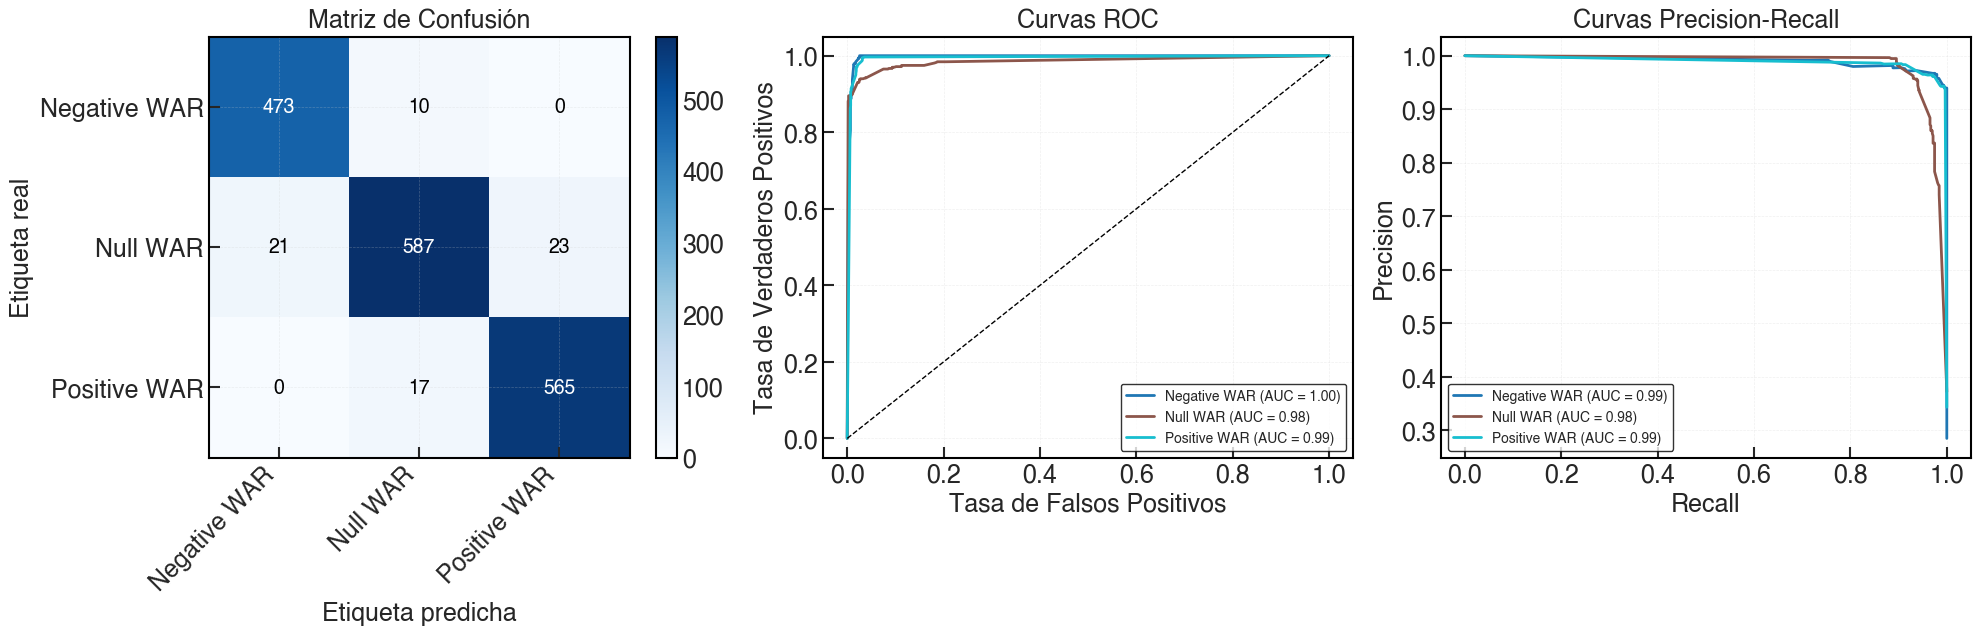
\includegraphics[width=0.8\linewidth]{figures//p2/roc_pr_random_forest_test.png}
    \caption{Resumen gráfico de métricas del modelo entrenado con Random Forest y evaluado sobre el conjunto de prueba.}
    \label{fig:roc_pr_random_forest_test}
\end{figure}


\subsection{Tablas}


\begin{table}[H]
\centering
\caption{Desempeño de modelos sobre el conjunto de prueba \texttt{WAR\_class\_test} }
\label{tab:metrics_war_class}
\begin{tabular}{lcccc}
\toprule
\textbf{Modelo} & \textbf{Accuracy} & \textbf{Precision} & \textbf{Recall} & \textbf{F1 Score} \\
\midrule
Regresión Logística Multiclase & 0.8874 & 0.8956 & 0.8874 & 0.8836 \\
LDA (solver='svd') & 0.9051 & 0.9145 & 0.9051 & 0.9020 \\
Random Forest (T=3) & \textbf{0.9581} & \textbf{0.9581} & \textbf{0.9581} & \textbf{0.9580} \\
\bottomrule
\end{tabular}
\end{table}

\begin{table}[H]
\centering
\caption{Desempeño de modelos sobre el conjunto de validación}
\label{tab:val_war_class}
\begin{tabular}{lcccc}
\toprule
\textbf{Modelo} & \textbf{Accuracy} & \textbf{Precision} & \textbf{Recall} & \textbf{F1 Score} \\
\midrule
Regresión Logística Multiclase & 0.6041 & 0.4218 & 0.6041 & 0.4965 \\
LDA (solver='svd') & 0.9232 & 0.9322 & 0.9232 & 0.9215 \\
Random Forest (T=3) & \textbf{0.9845} & \textbf{0.9847} & \textbf{0.9845} & \textbf{0.9845} \\
\bottomrule
\end{tabular}
\end{table}


\section{Imputación con KNN}
\label{subsec:knn}

Para el tratamiento de valores faltantes en variables numéricas, se utilizó el algoritmo \textit{K-Nearest Neighbors} (KNN). Este método imputa valores ausentes en función de las observaciones más similares (vecinas), calculadas mediante una métrica de distancia. En este trabajo, se empleó la distancia euclidiana:

\begin{equation}
d(\mathbf{x}, \mathbf{y}) = \sqrt{\sum_{i=1}^{n} (x_i - y_i)^2},
\end{equation}

donde \(\mathbf{x}\) y \(\mathbf{y}\) son vectores de características de dos observaciones, e \(n\) representa el número de atributos considerados. 


% Descripción del procedimiento KNN

\section{Winsorización por IQR}
\label{subsec:iqr}



Los valores atípicos fueron identificados mediante el método del rango intercuartílico (IQR), una técnica robusta basada en estadísticos de posición. Dado un conjunto de datos, se calcularon los cuartiles \(Q_1\) (percentil 25) y \(Q_3\) (percentil 75), definiendo el IQR como:

\begin{equation}
IQR = Q_3 - Q_1.
\end{equation}

Los umbrales para considerar un valor como atípico fueron:

\begin{equation}
L_{\text{inf}} = Q_1 - 1.5 \times IQR, \quad L_{\text{sup}} = Q_3 + 1.5 \times IQR.
\end{equation}

Los valores fuera de este rango fueron considerados outliers y tratados mediante winsorización, es decir, se truncaron al valor del límite más próximo (\(L_{\text{inf}}\) o \(L_{\text{sup}}\)). Esta técnica conserva todas las observaciones, pero limita el impacto de valores extremos sobre el modelo, estabilizando las distribuciones sin alterar la cantidad de datos disponibles.

Este procedimiento fue aplicado a todas las variables numéricas clave antes del entrenamiento de modelos predictivos.




\section{Métricas de Desempeño}\label{subsec:metricas-desempenio}

Para medir el rendimiento, se emplearon las métricas clásicas de clasificación: precisión, recall, F1-score, exactitud, AUC-ROC y AUC-PR. La precisión se define como:

\begin{equation}
\text{Precision} = \frac{TP}{TP + FP},
\end{equation}

el recall como:

\begin{equation}
\text{Recall} = \frac{TP}{TP + FN},
\end{equation}

el F1-score como:

\begin{equation}
F1 = 2 \cdot \frac{\text{Precision} \cdot \text{Recall}}{\text{Precision} + \text{Recall}},
\end{equation}

y la exactitud como:

\begin{equation}
\text{Accuracy} = \frac{TP + TN}{TP + TN + FP + FN}.
\end{equation}

Las curvas ROC y PR fueron construidas variando el umbral de decisión. Las áreas bajo dichas curvas (AUC) se utilizaron como indicadores de desempeño global.



% Bibliografía
% \bibliographystyle{plain}`'
% \bibliography{bibliografia}

\end{document}




